\section{Kommentarer}\label{kommentarer}

 Som nævnt i userstorien: "Kommentering af annonce" skal der kunne kommenteres annoncer. Der er derfor i modellen oprettet en kommentar klasse, der indeholder \begin{itemize}
 	\item Den aktuelle bytteannonce
 	\item Oprettelsestidspunkt
 	\item Kommentarteksten (Maximalt 500 tegn)
 	\item Den kommenterende bruger 
 \end{itemize}    
 
 Controlleren opretter automatisk værdierne, til at gemme i modellen. Viewet er lavet så det benytter et Http POST kald som tager kommentaren i tekstfeltet som ses på figur \ref{fig:Kommentar}. Ved klik på submit sendes dette kald.
 
 \begin{figure}[H]
 	\centering
 	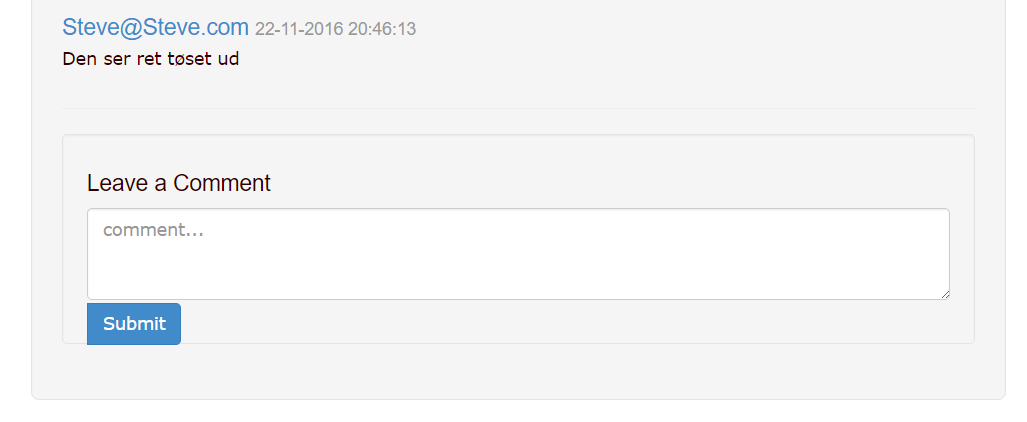
\includegraphics
 	[width=140mm]{../Dokumentation/figures/Kommentar.PNG}
 	\caption{Udseende af kommentarer}
 	\label{fig:Kommentar}
 \end{figure}
 
 Dette gemmes i databasen og alle kommentarer vises i rækkefølge, på viewet. Yderligere information om hvordan logikken i dette virker, kan findes i Design og implemenering.  